% !TeX root = ../Book2.tex
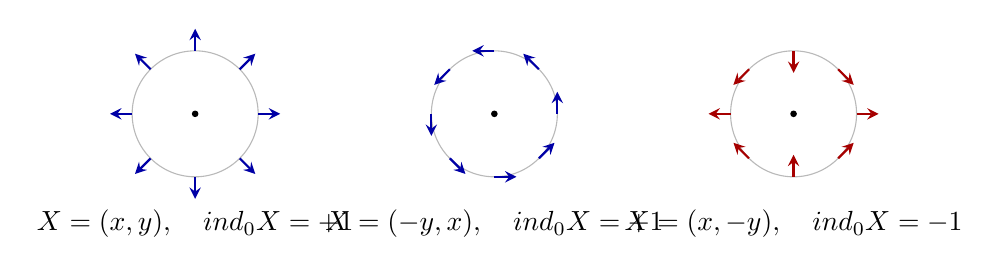
\begin{tikzpicture}[>=stealth]
	\foreach \shift/\kind/\formula/\value in {0/0/{(x,y)}/+1,3.8/1/{(-y,x)}/+1,7.6/2/{(x,-y)}/-1} {
		\begin{scope}[xshift=\shift cm]
			\draw[gray!55] (0,0) circle (0.8);
			\fill (0,0) circle (1.2pt);
			\foreach \a in {0,45,...,315} {
				\pgfmathsetmacro{\px}{0.8*cos(\a)}
				\pgfmathsetmacro{\py}{0.8*sin(\a)}
				\ifnum\kind=0
					\draw[->,thick,blue!65!black] (\px,\py)--({\px+0.28*cos(\a)},{\py+0.28*sin(\a)});
				\else\ifnum\kind=1
					\draw[->,thick,blue!65!black] (\px,\py)--({\px-0.28*sin(\a)},{\py+0.28*cos(\a)});
				\else
					\draw[->,thick,red!65!black] (\px,\py)--({\px+0.28*cos(\a)},{\py-0.28*sin(\a)});
				\fi\fi
			}
			\node at (0,-1.4) {\(X=\formula,\quad\operatorname{ind}_0X=\value\)};
		\end{scope}
	}
\end{tikzpicture}
